%%%%%%%%%%%%%%%%%%%%%%%%%%%%%%%%%%%%%%%%%
% Beamer Presentation
% LaTeX Template
% Version 1.0 (10/11/12)
%
% This template has been downloaded from:
% http://www.LaTeXTemplates.com
%
% License:
% CC BY-NC-SA 3.0 (http://creativecommons.org/licenses/by-nc-sa/3.0/)
%
%%%%%%%%%%%%%%%%%%%%%%%%%%%%%%%%%%%%%%%%%

%-------------------------------------------------------------------------------
%	PACKAGES AND THEMES
%-------------------------------------------------------------------------------

\documentclass{beamer}
\usepackage{xcolor}
\usepackage{graphicx}
\usepackage{tikz}
\usepackage{listings}
\usepackage{multicol}

\DeclareMathOperator{\diag}{diag}

\definecolor{applegreen}{rgb}{0.55, 0.71, 0.0}
\definecolor{blue(ncs)}{rgb}{0.0, 0.45, 0.60}
\definecolor{burgundy}{rgb}{0.5, 0.0, 0.13}

\definecolor{cadet}{rgb}{0.33, 0.41, 0.47}
\definecolor{airforceblue}{rgb}{0.36, 0.54, 0.66}

\mode<presentation> {

\usetheme{CambridgeUS}

\usecolortheme{wolverine}

\definecolor{gold}{HTML}{D4A017}
\definecolor{darkgold}{HTML}{B7950B}

\setbeamercolor{palette primary}{bg=cadet,fg=white}
\setbeamercolor{palette secondary}{bg=airforceblue,fg=white}
\setbeamercolor{palette tertiary}{bg=black,fg=white}
\setbeamercolor{palette quaternary}{bg=cadet,fg=white}

\setbeamercolor{frametitle}{bg=airforceblue,fg=white}

\setbeamercolor{section number projected}{bg=black,fg=cadet}
\setbeamercolor{item}{fg=black,bg=cadet}

\setbeamertemplate{page number in head/foot}[framenumber]

\lstset{basicstyle=\ttfamily\footnotesize,breaklines=true}
}

\lstdefinestyle{yaml}{
     basicstyle=\color{blue}\footnotesize\ttfamily,
     rulecolor=\color{black},
     string=[s]{'}{'},
     stringstyle=\color{blue},
     comment=[l]{:},
     commentstyle=\color{black},
     morecomment=[l]{-},
     numbers=left,
     firstnumber=auto,
     numberblanklines=true,
     frame=trbL,
     numberstyle=\tiny,
     frame=leftline,
     numbersep=7pt,
     framesep=5pt,
     framerule=10pt,
     xleftmargin=15pt,
     backgroundcolor=\color[gray]{0.97},
     rulecolor=\color[gray]{0.90}%
}

\usepackage{graphicx} % Allows including images
\usepackage{booktabs} % Allows the use of \toprule, \midrule and \bottomrule in tables

%----------------------------------------------------------------------------------------
%	TITLE PAGE
%----------------------------------------------------------------------------------------

\title[Ratel]{Matrix-Free MPM on High-Order Meshes with Ratel and libCEED} % The short title appears at the bottom of every slide, the full title is only on the title page

\author{Jeremy L Thompson} % Your name
\institute[CU Boulder] % Your institution as it will appear on the bottom of every slide, may be shorthand to save space
{University of Colorado Boulder \\ % Your institution for the title page
\medskip
\textit{jeremy@jeremylt.org} % Your email address
}
\date{15 July 2025} % Date, can be changed to a custom date

\begin{document}

\begin{frame}
\titlepage % Print the title page as the first slide
\end{frame}
 
%------------------------------------------------

\begin{frame}
\frametitle{Ratel Team}

\begin{center}
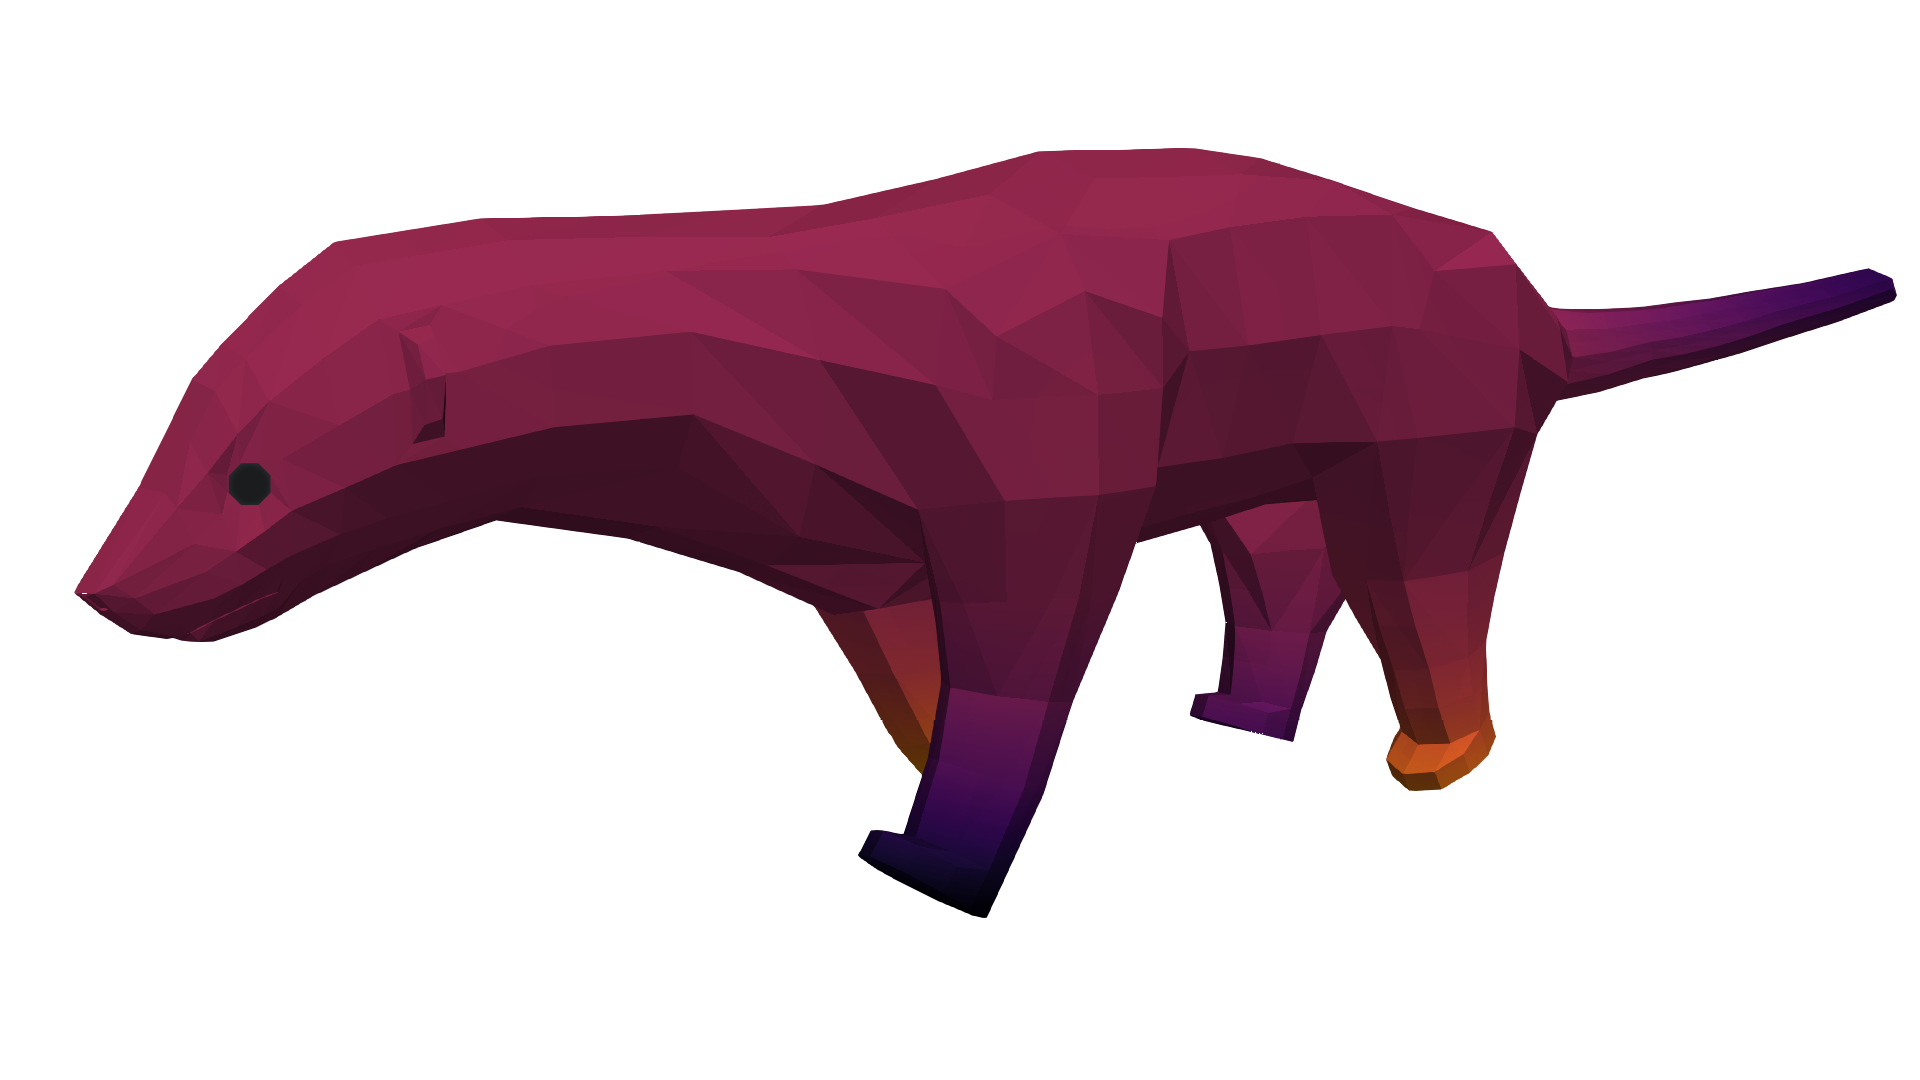
\includegraphics[height=2.75cm]{Ratellogo.png}
\end{center}

{\flushleft

Repository: https://gitlab.com/micromorph/ratel\\

~\\

Developers: Zach R. Atkins, Jed Brown, Fabio Di Gioacchino,\\
\hspace{19mm} Leila Ghaffari, Zach Irwin, Rezgar Shakeri,\\
\hspace{19mm} Ren Stengel, Jeremy L Thompson\\

The authors acknowledge support by the Department of Energy, National Nuclear Security Administration, Predictive Science Academic Alliance Program (PSAAP) under Award Number DE-NA0003962.

}

\begin{center}

\includegraphics[height=0.7cm]{psaap-center-logos}
\end{center}

\end{frame}

%------------------------------------------------

\begin{frame}
\begin{center}
\frametitle{Overview}

Ratel - high order, performance portable solid mechanics\\

~\\

Built on libCEED and PETSc\\

~\\

GPU and CPU performance\\

~\\

\end{center}
\end{frame}
 
%------------------------------------------------

\begin{frame}
\frametitle{Overview} % Table of contents slide, comment this block out to remove it
\tableofcontents % Throughout your presentation, if you choose to use \section{} and \subsection{} commands, these will automatically be printed on this slide as an overview of your presentation
\end{frame}

%------------------------------------------------
\section{Ratel Background}
%------------------------------------------------

\begin{frame}
\begin{center}
\frametitle{ECP Roots}

\begin{itemize}

\item Ratel built directly on results from ECP CEED project\\

~\\

\item libCEED provides high-performance operator evaluation\\

~\\

\item PETSc provides linear/non-linear solvers and time steppers\\

~\\

\item Ratel built from libCEED + PETSc solid mechanics demo app\\

\end{itemize}

\end{center}
\end{frame}

%------------------------------------------------

\begin{frame}
\begin{center}
\frametitle{Matrix-Free Operators from libCEED}

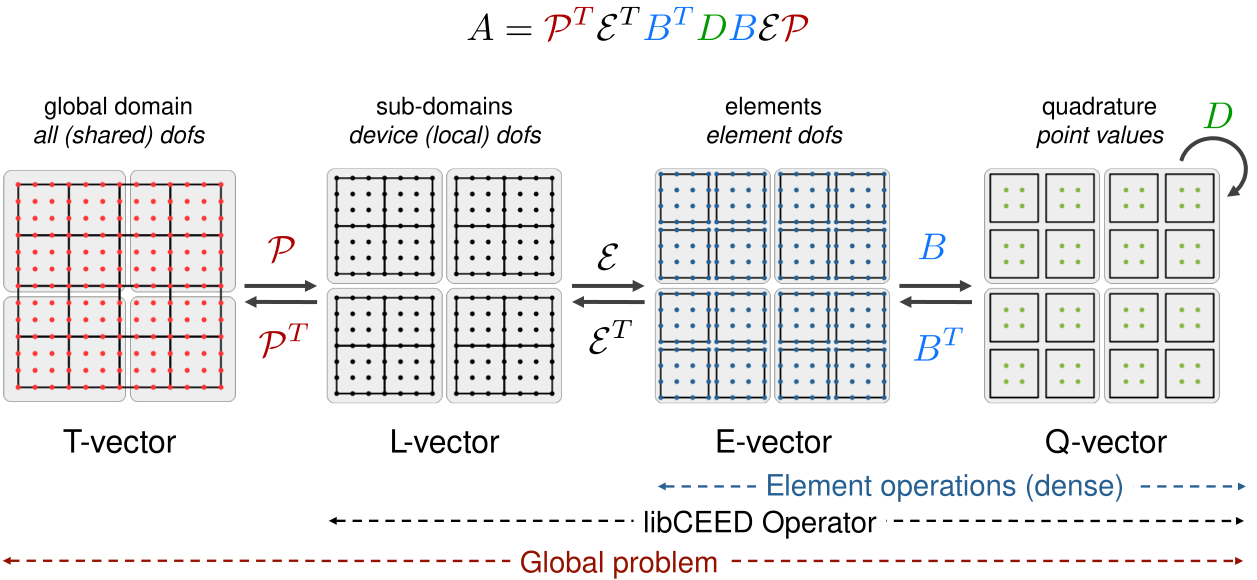
\includegraphics[height=5.0cm]{libCEEDAPI.png}

~\\

libCEED provides arbitrary order matrix-free operator evaluation\\

\end{center}
\end{frame}

%------------------------------------------------

\begin{frame}
\begin{center}
\frametitle{Performance Portability from libCEED}

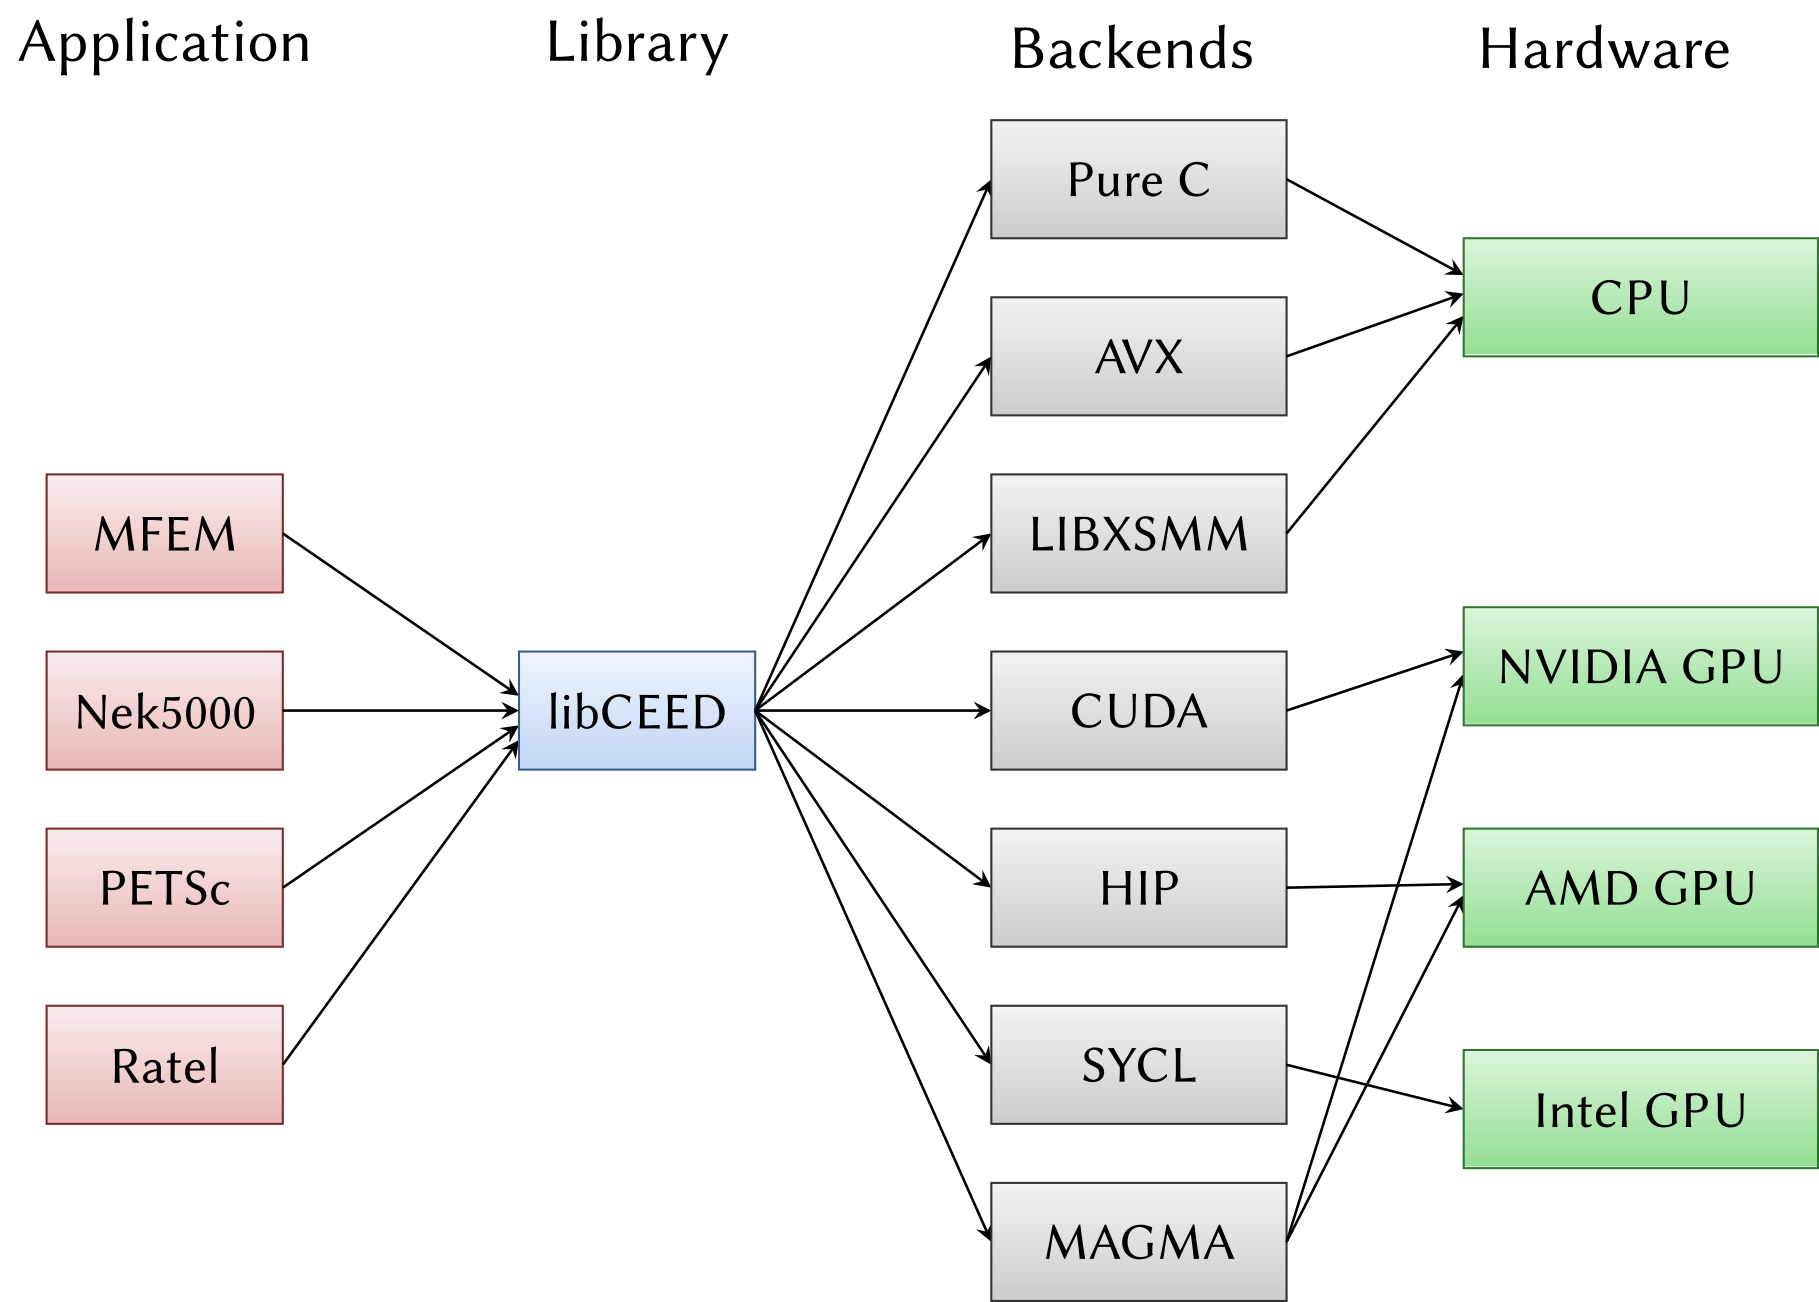
\includegraphics[height=5.5cm]{libCEEDBackends.png}

~\\

Performance portability with libCEED's matrix-free operators\\

\end{center}
\end{frame}

%------------------------------------------------

\begin{frame}
\begin{center}
\frametitle{Extensible Solvers from PETSc}

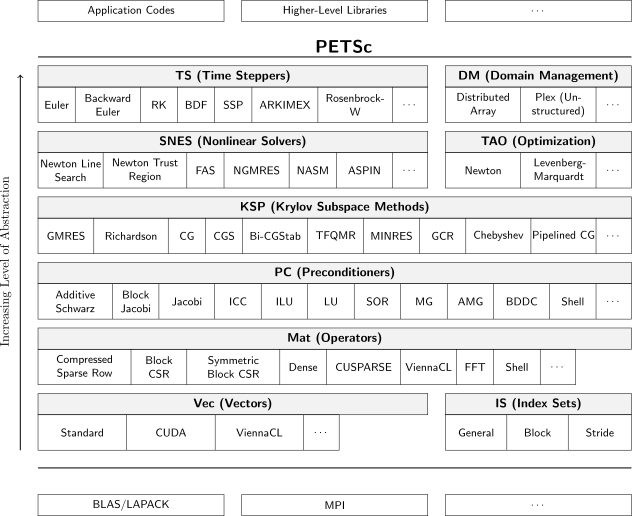
\includegraphics[height=6.0cm]{PETScAPI.png}

~\\

PETSc provides extensible, scalable solvers\\

\end{center}
\end{frame}

%------------------------------------------------
\section{AtPoints Evaluation}
%------------------------------------------------

\begin{frame}
\begin{center}
\frametitle{What is MPM?}

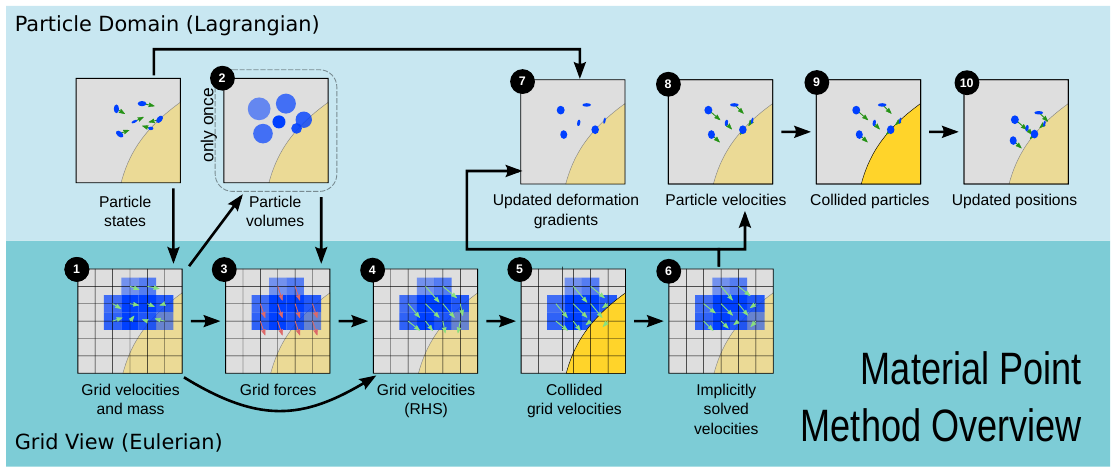
\includegraphics[height=5cm]{MPMOverview.png}\\

~\\

\begin{itemize}

\item Continuum based particle method with background mesh for gradients\\

\item Extension of FLIP (which is an extension of PIC)\\

\item Enables large deformation simulations with complex features\\

\end{itemize}

\end{center}
\end{frame}

%------------------------------------------------

\begin{frame}
\begin{center}
\frametitle{MPM vs FEM}

MPM can be formulated as very similar to FEM\\

~\\

\begin{itemize}

\item Problem on background mesh changes when material points move\\

~\\

\item Can be viewed as FEM with arbitrary quadrature point locations\\

~\\

\item Natural fit for libCEED matrix-free representation\\

~\\

\item Ratel FEM infrastructure provides fast background mesh solves\\

\end{itemize}

\end{center}
\end{frame}

%------------------------------------------------

\begin{frame}
\begin{center}
\frametitle{libCEED Basis Evaluation to Points}

\begin{center}
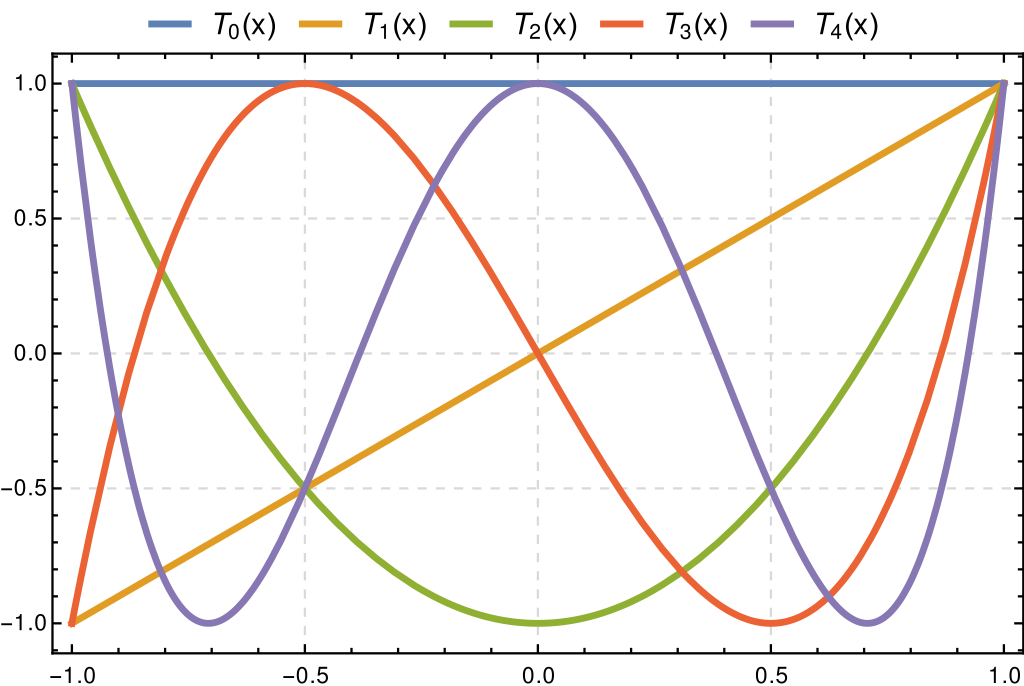
\includegraphics[height=4cm]{ChebyshevPolynomials.png}
\end{center}

\begin{itemize}

\item Interpolate from primal to dual (quadrature) space\\

~\\

\item Fit Chebyshev polynomials to values at quadrature points\\

~\\

\item Evaluate Chebyshev polynomials at arbitrary points\\

\end{itemize}

\end{center}
\end{frame}

%------------------------------------------------

\begin{frame}
\begin{center}
\frametitle{libCEED Basis Evaluation to Points}

Interpolation to Chebyshev has same FLOPs as FEM $\mathcal{O} \left( q^4 \right)$

~\\

\begin{itemize}

\item Invert map $C^{-1}$ from quadrature points to Chebyshev coeffs\\

~\\

\item Create 1D interpolation matrix $B = C N$\\

~\\

\item Tensor product: $B = \left( C \otimes C \otimes C \right) \left( N \otimes N \otimes N \right) = \left( C N \right) \otimes \left( C N \right) \otimes \left( C N \right)$\\

~\\

\item Additional cost from evaluation to arbitrary points\\

\end{itemize}

\end{center}
\end{frame}

%------------------------------------------------

\begin{frame}
\begin{center}
\frametitle{libCEED Basis Evaluation to Points}

Per point evaluation has higher FLOPs $\mathcal{O} \left( q^6 \right)$

~\\

\begin{itemize}

\item Recurrence for Chebyshev values at point\\

$f_0 = 1$, $f_1 = 2 x$, $f_n = 2 x f_{n - 1} - f_{n - 2}$\\

$f'_0 = 0$, $f'_1 = 2$, \hspace{0.7mm} $f'_n = 2 x f'_{n - 1} + 2 f_{n - 1} - f'_{n - 2}$\\

~\\

\item Contract pencil of values with element coefficients\\

~\\

\item Operation is independent per quadrature point\\

~\\

\item $\mathcal{O} \left( q^3 \right)$ FLOPs at $\mathcal{O} \left( q^3 \right)$ points\\

\end{itemize}

\end{center}
\end{frame}

%------------------------------------------------

\begin{frame}
\begin{center}
\frametitle{AtPoints Operator}

Final operator very similar to FEM\\

~\\

\begin{itemize}

\item $L = \mathcal{E}^T {\color{blue(ncs)} B^T} {\color{blue(ncs)} B^{e T}} {\color{applegreen} D} {\color{blue(ncs)} B^e} {\color{blue(ncs)} B} \mathcal{E}$ - CeedOperator\\

~\\

\item All other operations identical to FEM\\

~\\

\item libCEED gives action of local MPM operator\\

~\\

\item PETSc responsible for communication between devices\\

\hspace{6mm} $A = {\color{burgundy} P^T} L {\color{burgundy} P}$

\end{itemize}

\end{center}
\end{frame}

%------------------------------------------------

\begin{frame}
\begin{center}
\frametitle{Sample Run}

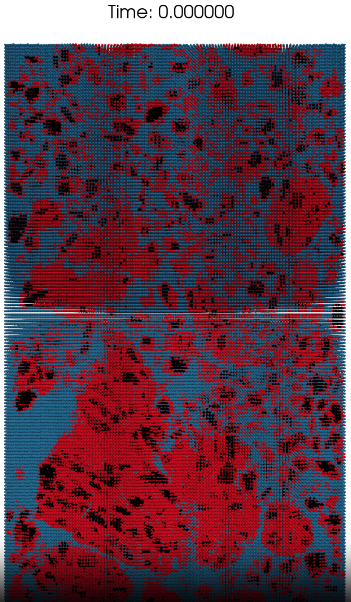
\includegraphics[height=6cm]{iMPM0.png}
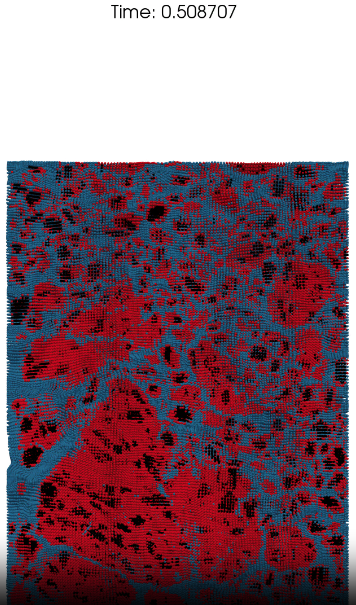
\includegraphics[height=6cm]{iMPM1.png}
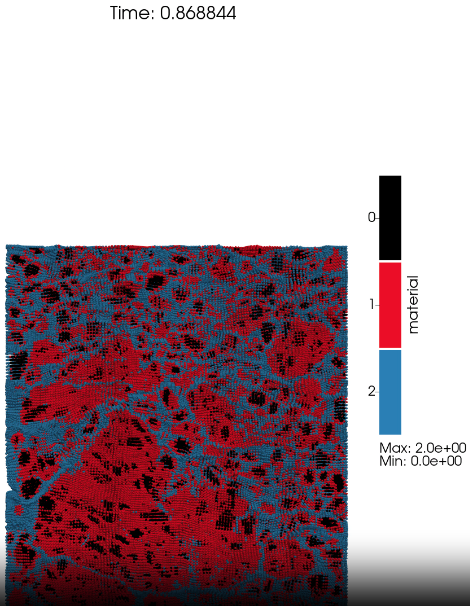
\includegraphics[height=6cm]{iMPM2.png}

Confined compression of mock HE material

\end{center}
\end{frame}

%------------------------------------------------
\section{Performance}
%------------------------------------------------

\begin{frame}
\begin{center}
\frametitle{CEED Benchmark Problems}

Performance on CEED BPs

~\\

\begin{itemize}

\item BP1 - Scalar projection problem\\

~\\

\item BP2 - 3 component projection problem\\

~\\

\item BP3 - Scalar Poisson problem\\

~\\

\item BP4 - 3 component Poisson problem\\

\end{itemize}

~\\

Bulk of FLOPs are in basis evaluation

\end{center}
\end{frame}

%------------------------------------------------

\begin{frame}
\begin{center}
\frametitle{CEED Benchmark Problems}

Performance on CEED BPs

~\\

\begin{itemize}

\item $p = 2, 3, 4$ and $q = p + 1$\\

~\\

\item Units cube with $30^3$, $60^3$, $90^3$, $120^3$, and $150^3$ elements\\

~\\

\item Compare tensor, non-tensor, and at-points basis evaluation\\

~\\

\item MMS w/ partial sum of Weierstrass function, $a = 0.5$, $b = 1.5$, $N = 2$\\

\end{itemize}

~\\

Using 4x AMD Instinct\texttrademark MI300A Accelerated Processing Units (APUs)

\end{center}
\end{frame}

%------------------------------------------------

\begin{frame}
\begin{center}
\frametitle{BP1}

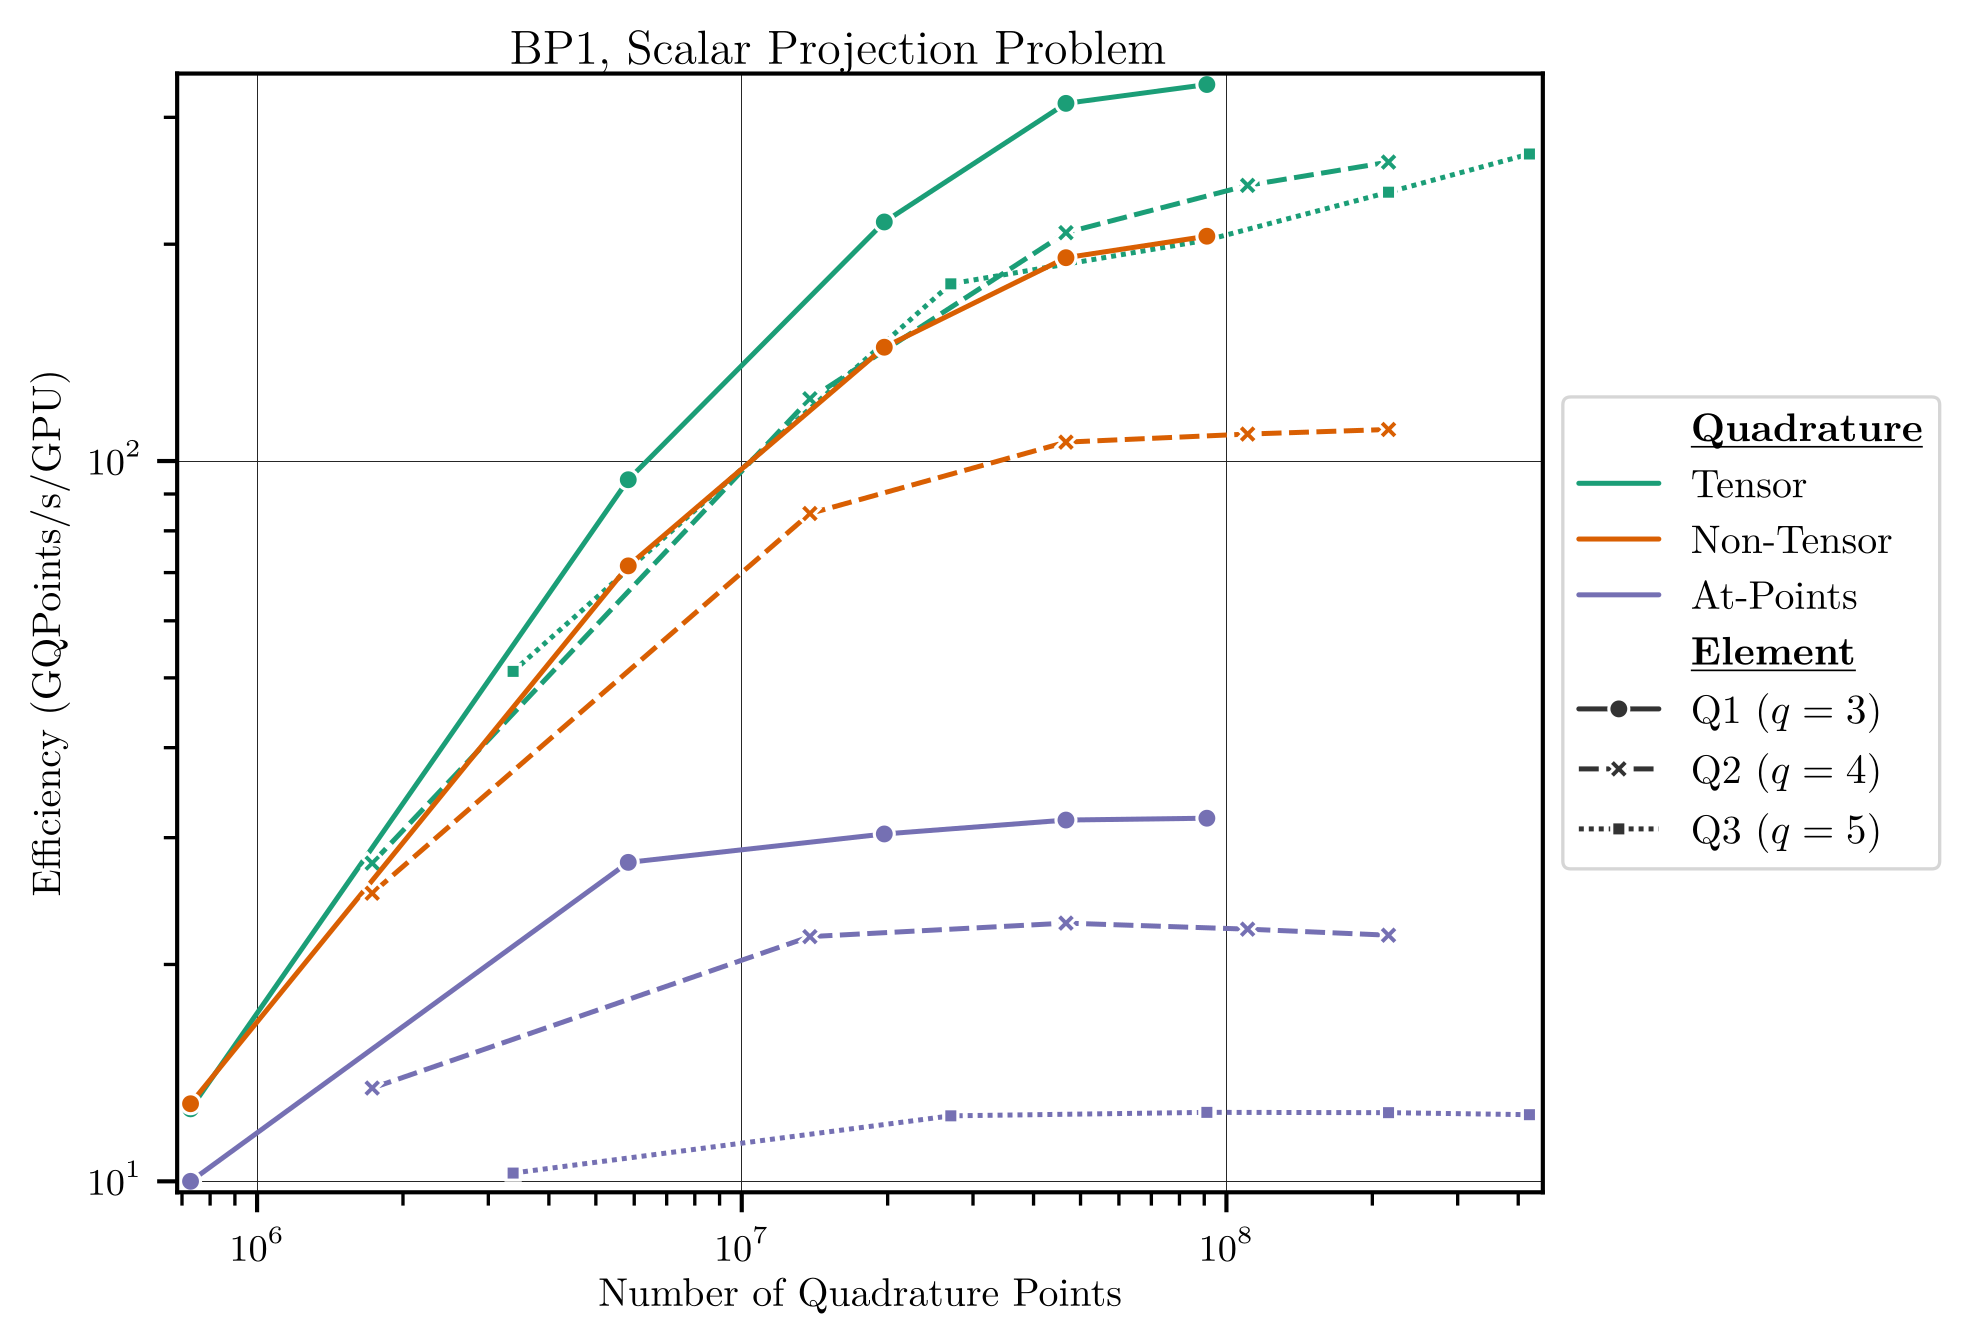
\includegraphics[height=6.5cm]{MPM_BP1.png}\\

~\\

More FLOPs leads to lower efficiency

\end{center}
\end{frame}

%------------------------------------------------

\begin{frame}
\begin{center}
\frametitle{BP2}

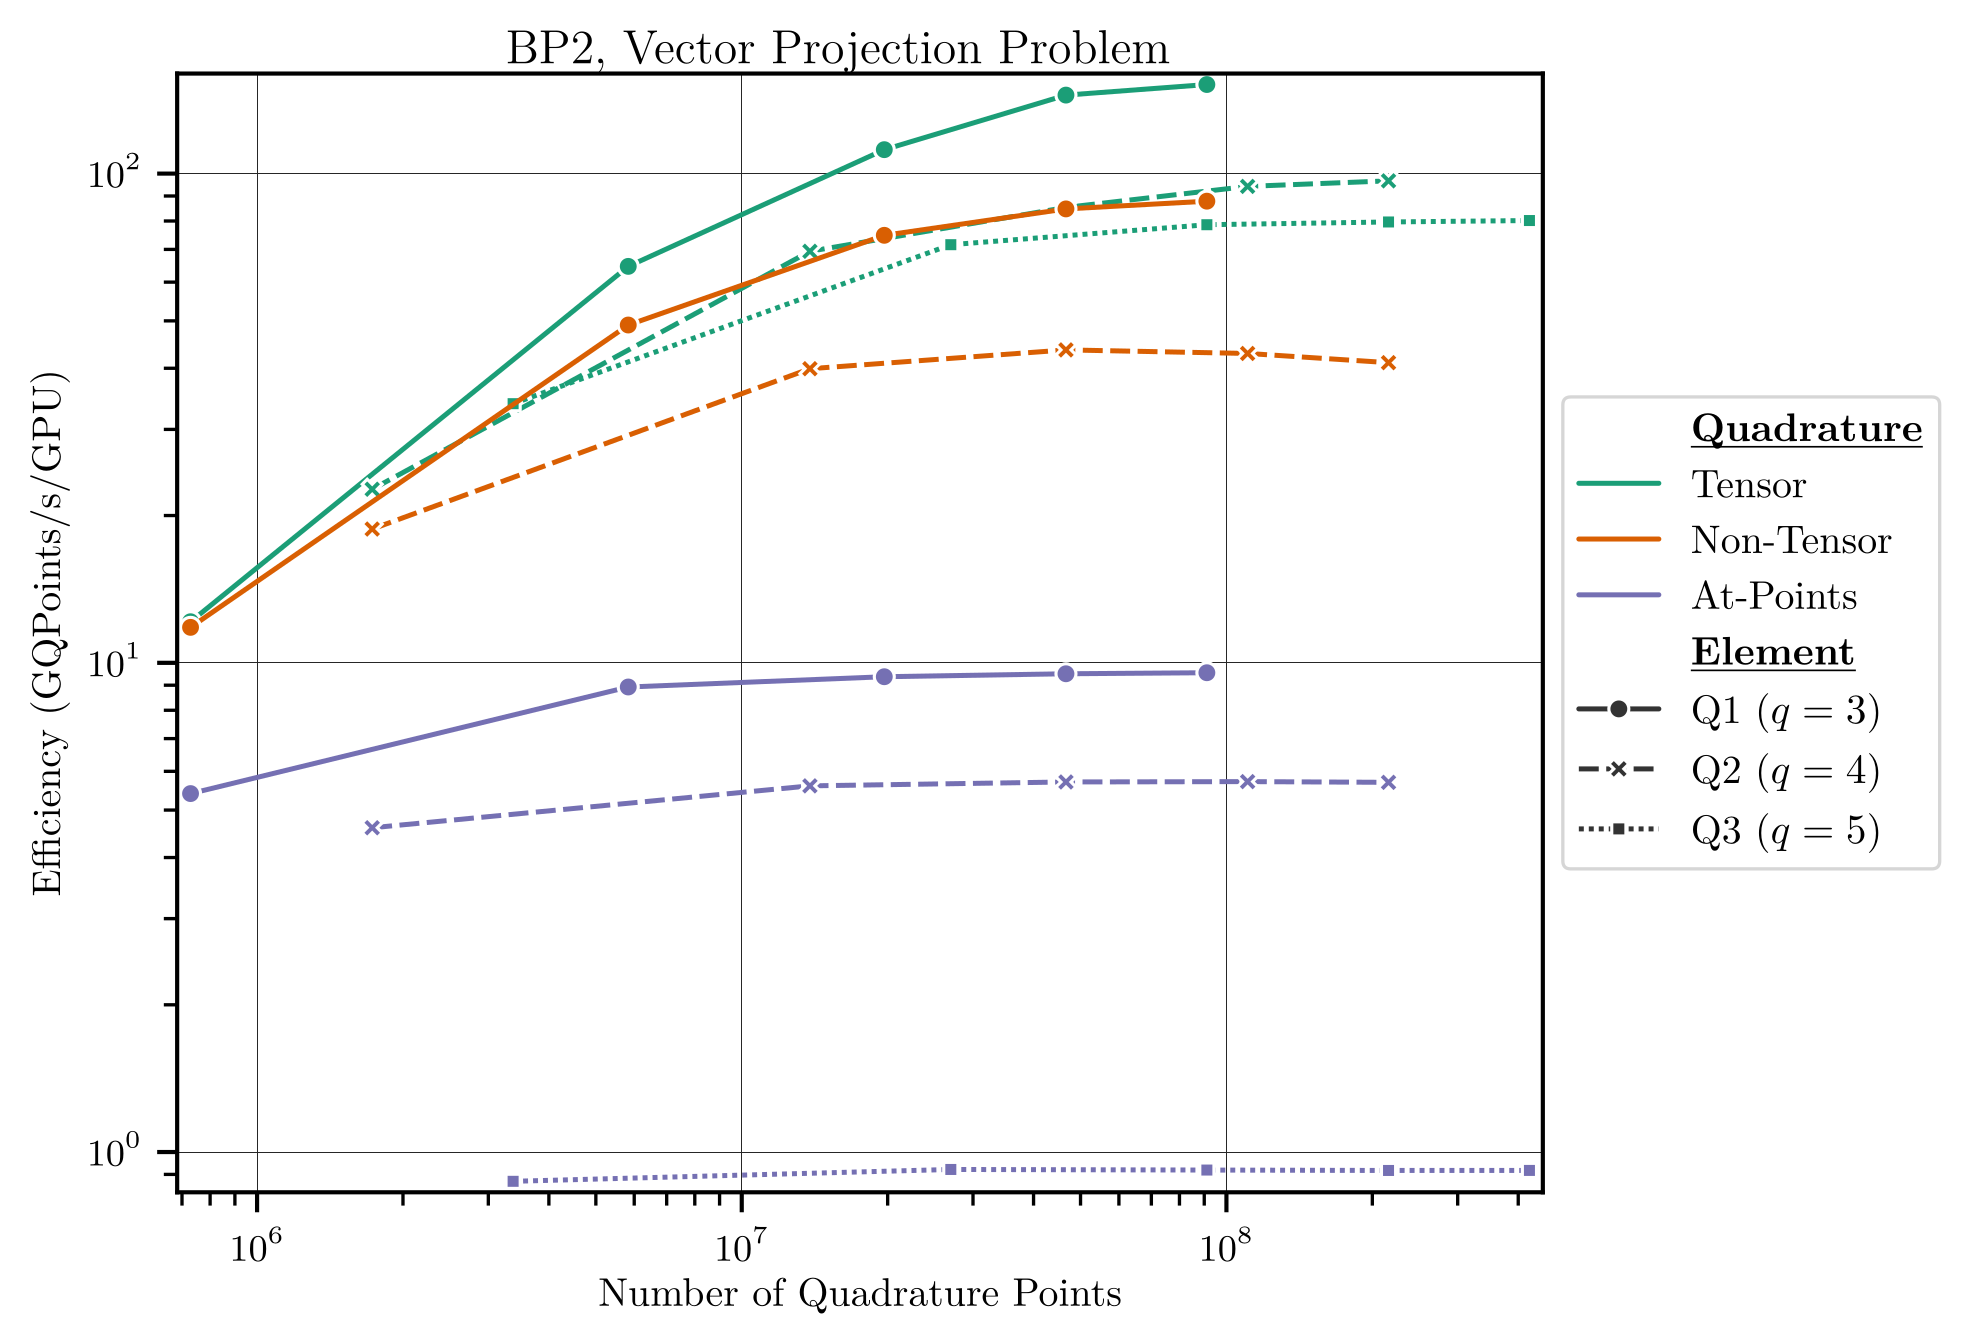
\includegraphics[height=6.5cm]{MPM_BP2.png}\\

~\\

With more components, reach peak efficiency faster

\end{center}
\end{frame}

%------------------------------------------------

\begin{frame}
\begin{center}
\frametitle{BP3}

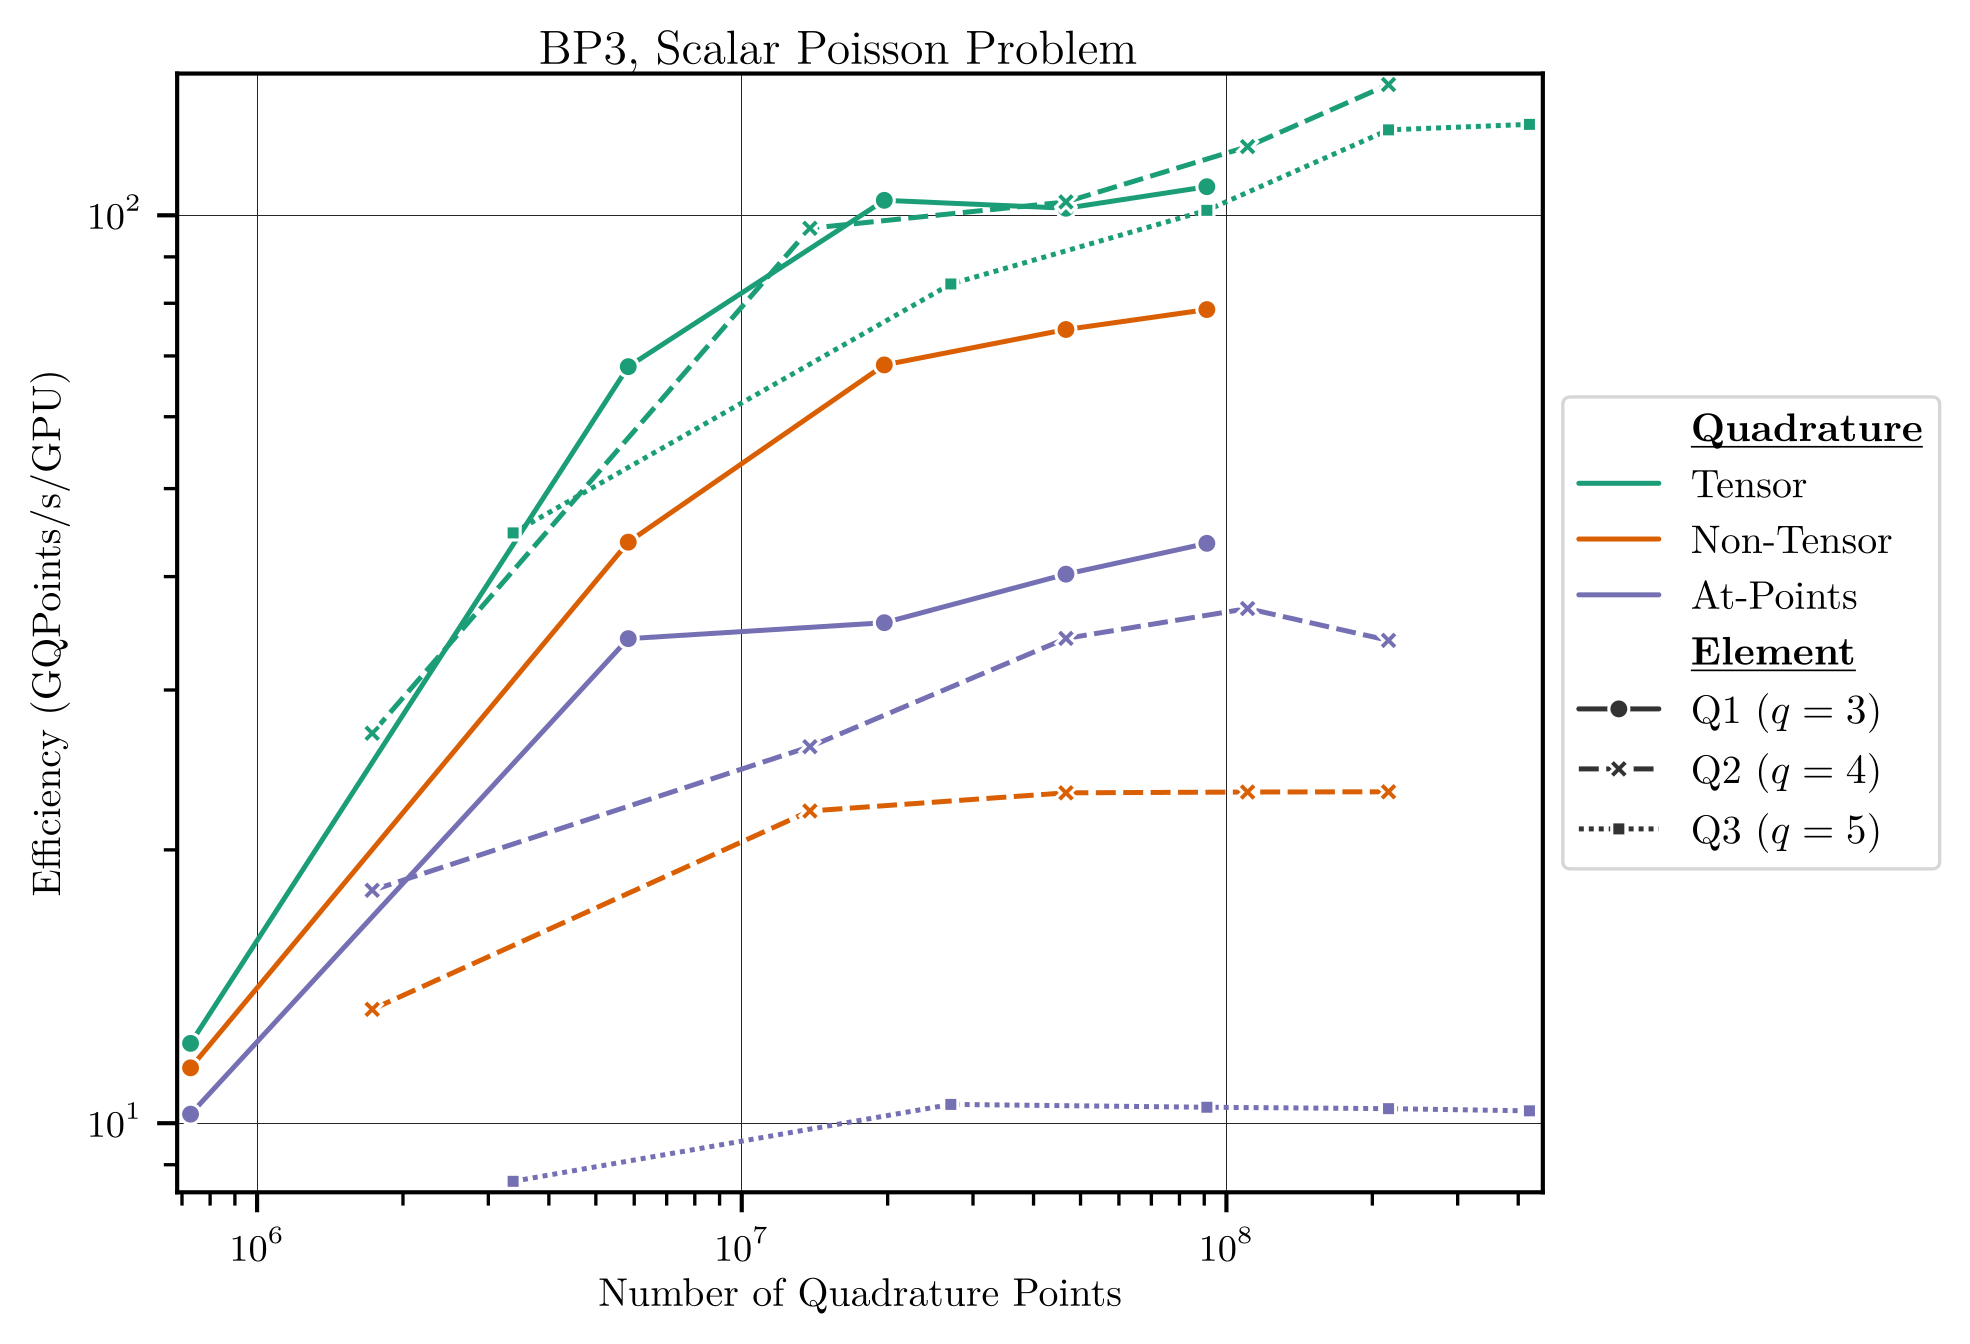
\includegraphics[height=6.5cm]{MPM_BP3.png}\\

~\\

With derivatives, at-points closer to non-tensor

\end{center}
\end{frame}

%------------------------------------------------

\begin{frame}
\begin{center}
\frametitle{BP3}

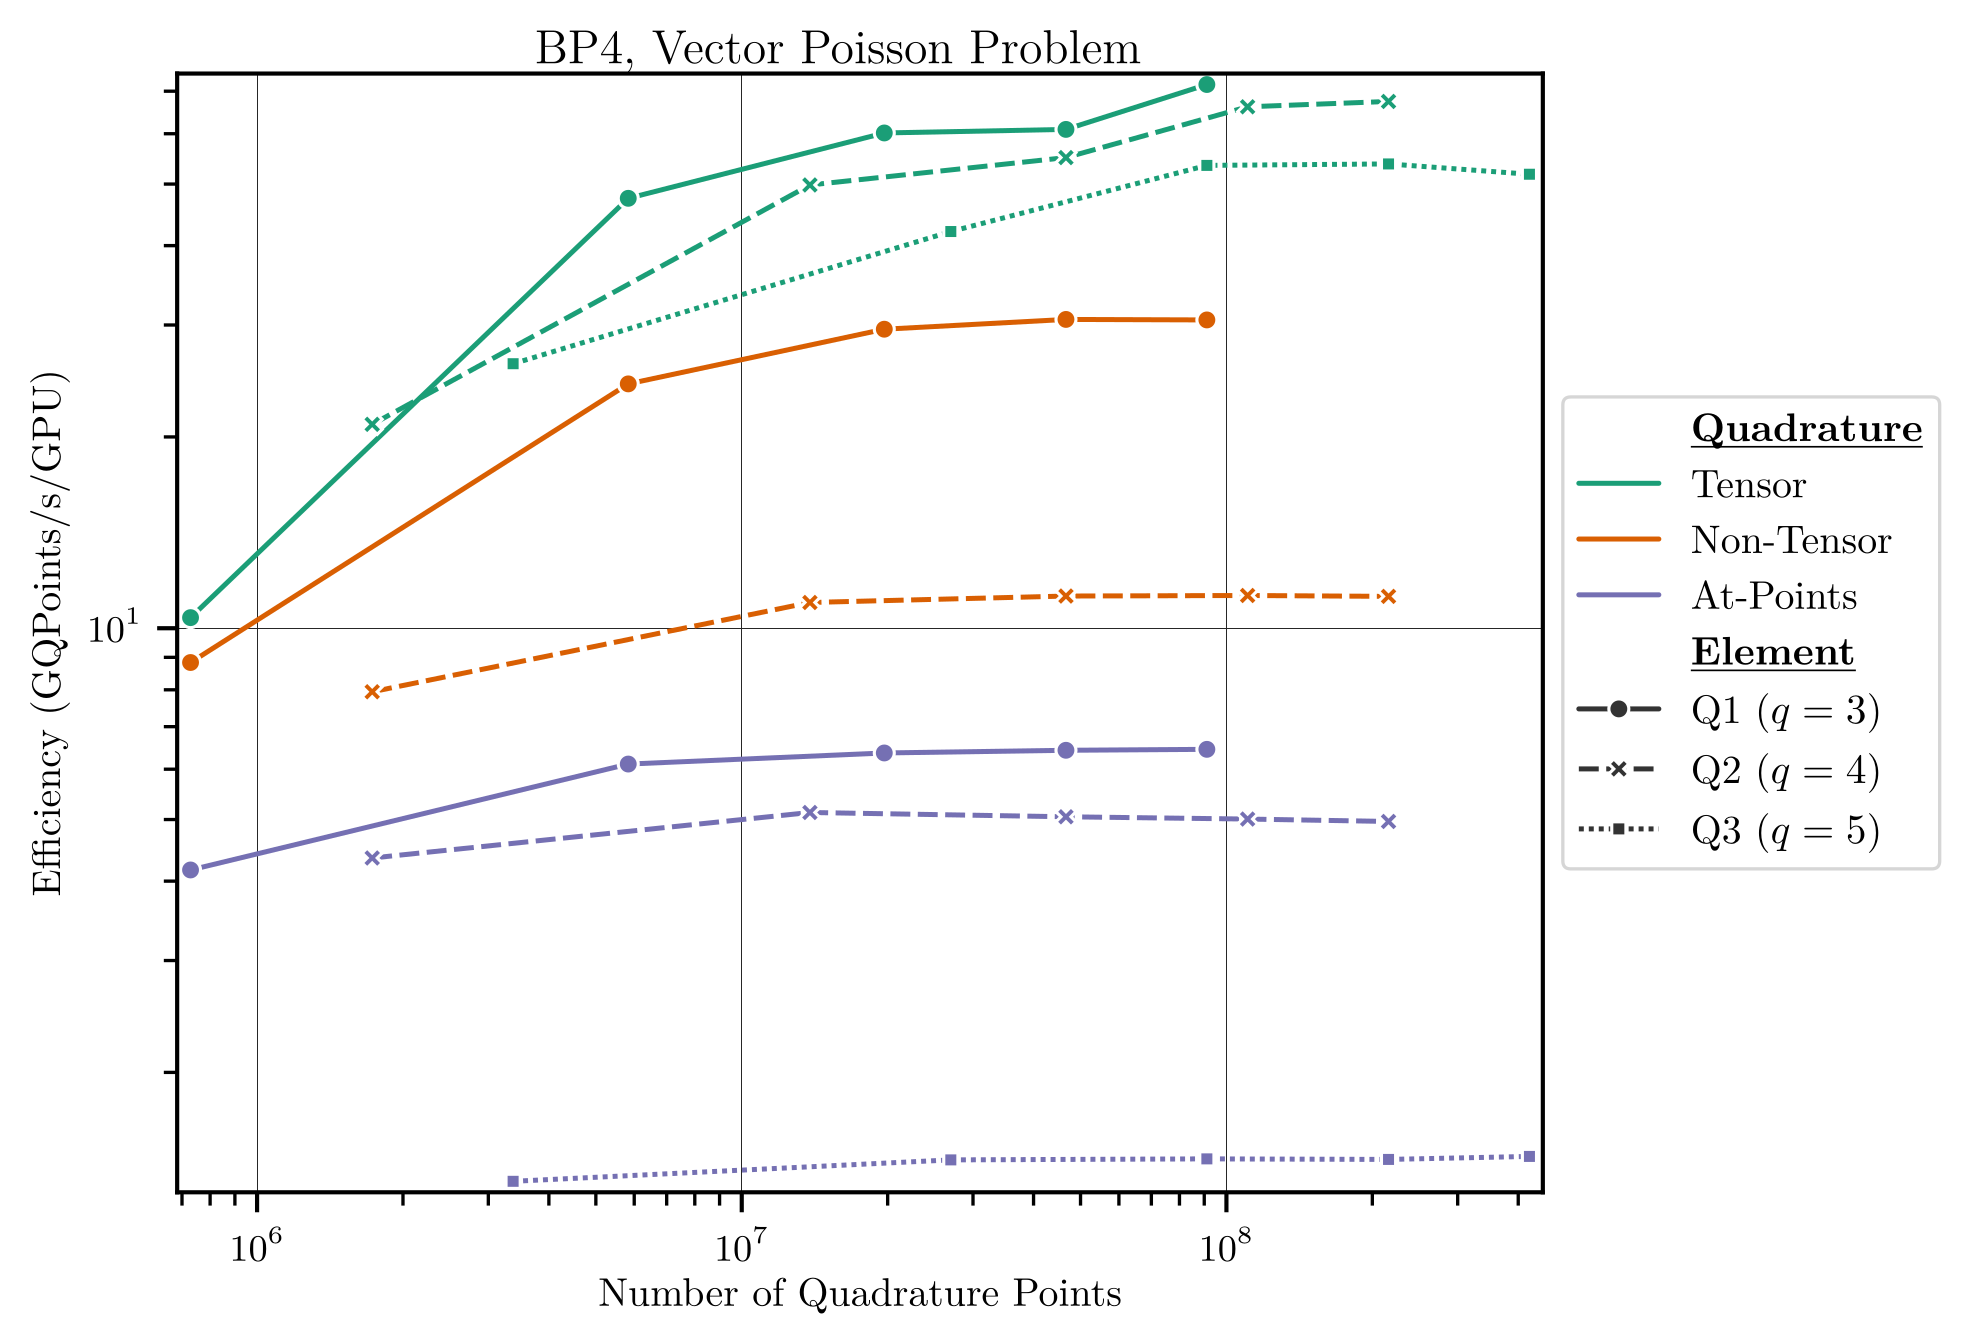
\includegraphics[height=6.5cm]{MPM_BP4.png}\\

~\\

Derivatives and more components worst for at-points

\end{center}
\end{frame}

%------------------------------------------------

\begin{frame}
\begin{center}
\frametitle{Ogden}

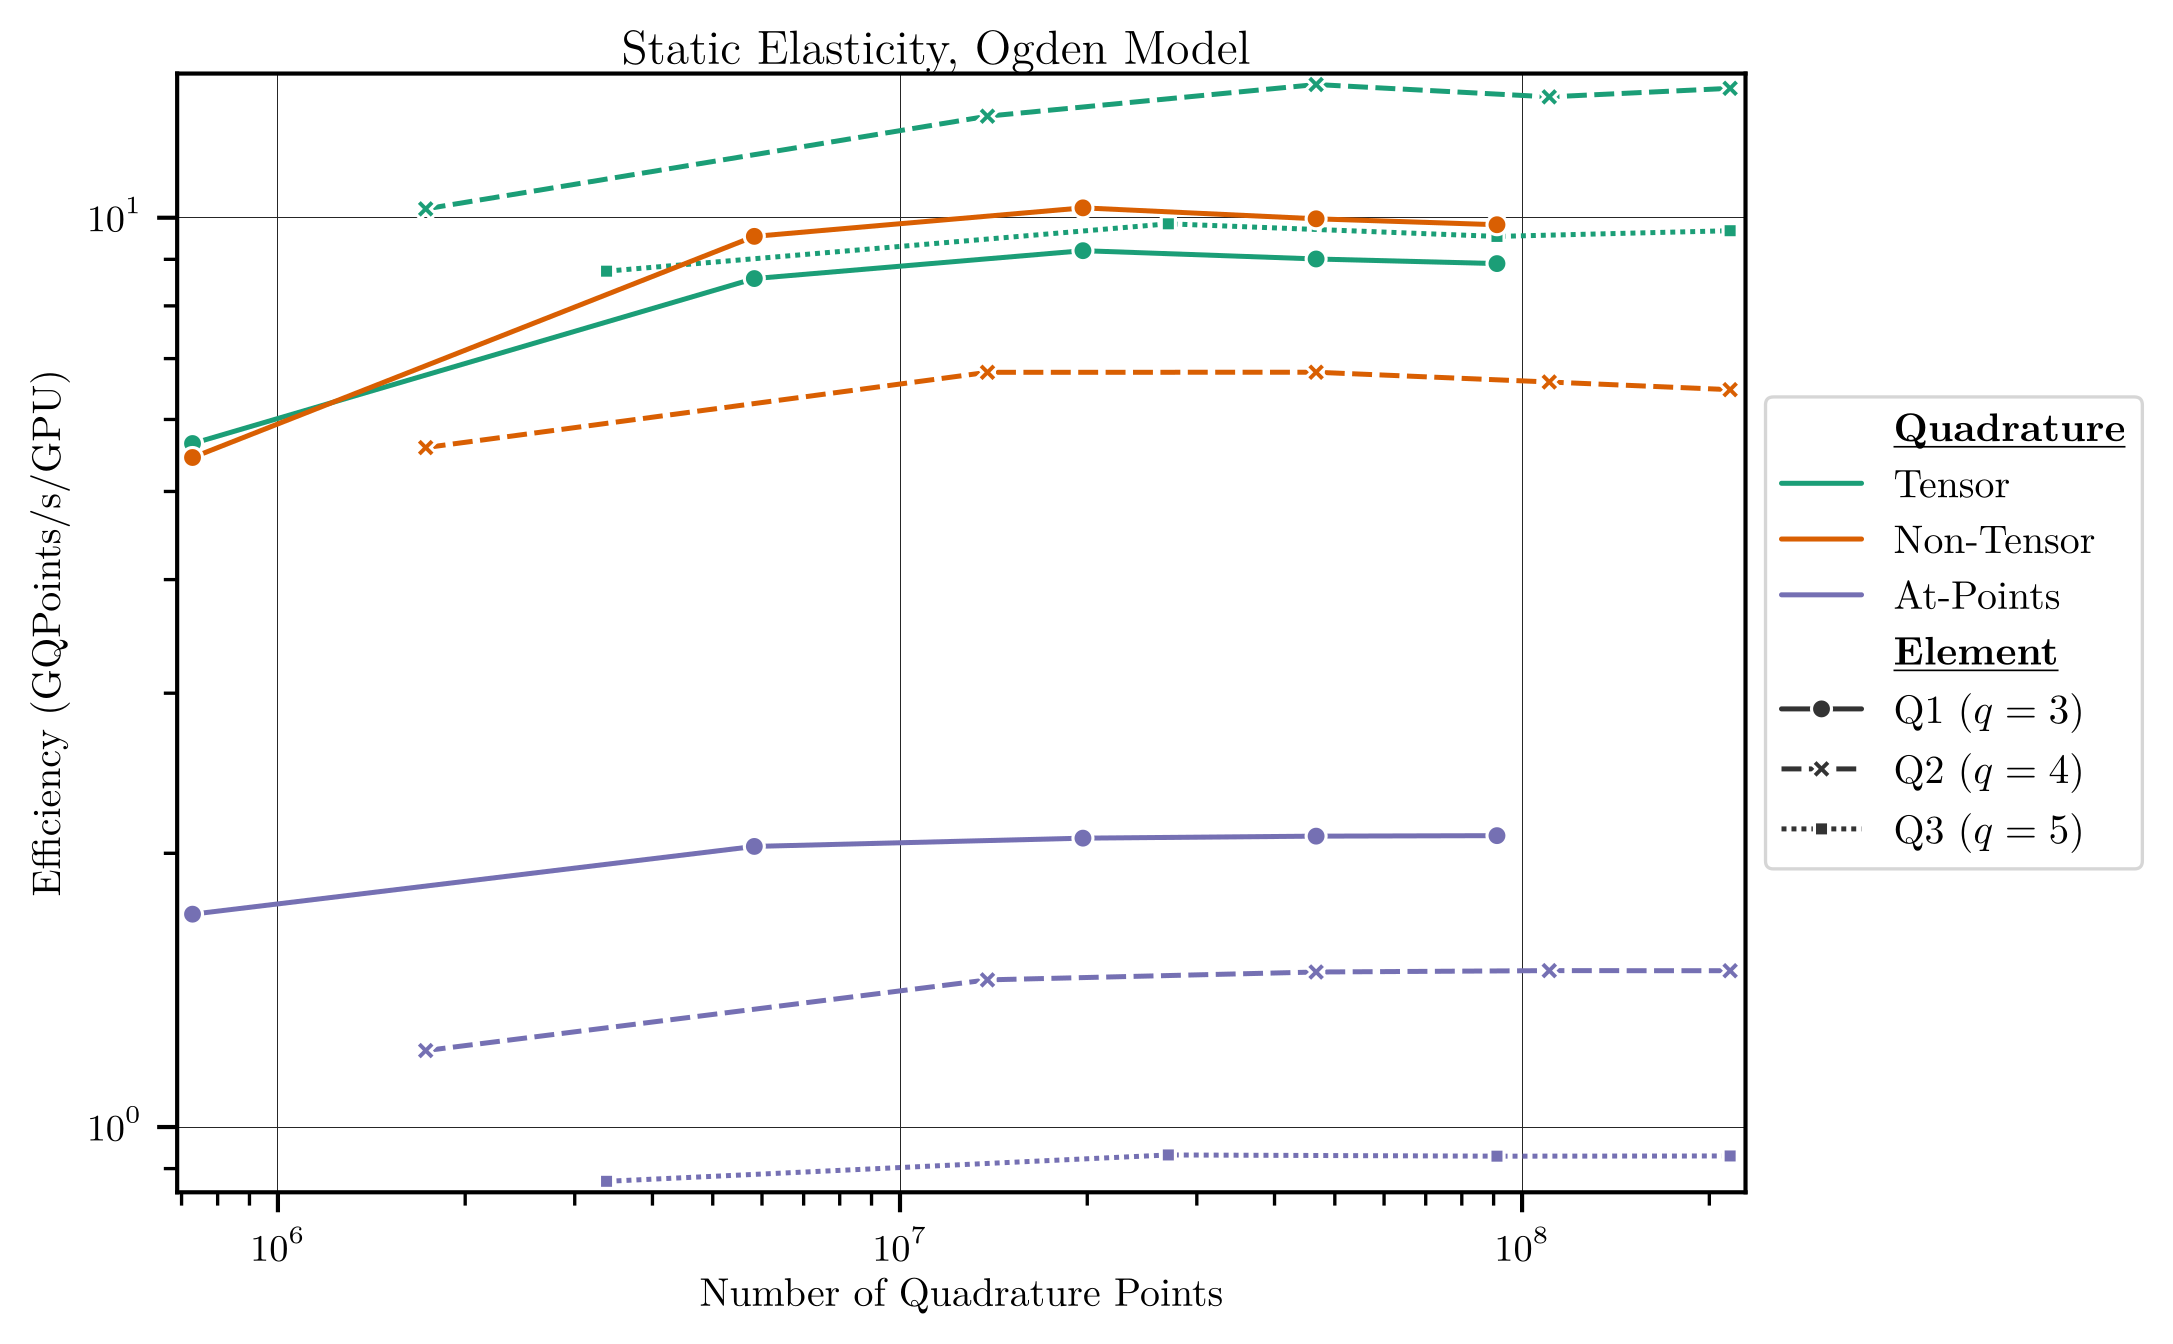
\includegraphics[height=6.5cm]{MPM_Ogden.png}\\

~\\

Still see cost with heavier QFunctions

\end{center}
\end{frame}

%------------------------------------------------
\section{Multigrid}
%------------------------------------------------

\begin{frame}
\begin{center}
\frametitle{Preconditioning}

Practical problems require preconditioning\\

~\\

\begin{itemize}

\item Problems for MPM tend to be poorly conditioned\\

~\\

\item Poor conditioning + expensive Mat-Vec = need preconditioning\\

~\\

\item Varying structure between elements makes assembly more difficult\\

\end{itemize}

\end{center}
\end{frame}

%------------------------------------------------

\begin{frame}
\begin{center}
\frametitle{PETSc PCMG}

\begin{itemize}

\item PCMG - PETSc geometric multigrid preconditioner\\

~\\

\item Requires several operators from the user\\

~\\

\begin{itemize}

\item Restriction operator\\

~\\

\item Interpolation operator\\

~\\

\item Smoother\\

~\\

\item Coarse grid solver

\end{itemize}

\end{itemize}

\end{center}
\end{frame}

%------------------------------------------------

\begin{frame}
\begin{center}
\frametitle{Ratel PCpMG}

2 level multigrid with PCpMG\\
~\\

\begin{tikzpicture}
\node[shape=circle,draw=black] (A) at (2,-2) {$p_f$};
\node[shape=circle] (Al) at (0.8,-2) {Smooth};
\node[shape=circle,draw=black] (B) at (4,-4) {$p_c$};
\node[shape=circle] (Bl) at (4,-5) {Coarse Solve (AMG)};
\node[shape=circle,draw=black] (C) at (6,-2) {$p_f$};
\node[shape=circle] (Cl) at (7.2,-2) {Smooth};
\path[->] (A) edge node[left=10, pos=.6] {Restriction} (B);
\path[->] (B) edge node[right=10, pos=.4] {Interpolation} (C);
\end{tikzpicture}

\end{center}
\end{frame}

%------------------------------------------------

\begin{frame}
\begin{center}
\frametitle{Ratel PCpMG}

pMG giving promising initial results with GPU impl\\

~\\

\begin{itemize}

\item Finite strain elasticity with damage\\

~\\

\item Confined press of grain/binder with "sticky air" voids\\

~\\

\item Jacobi iterations tend to double with 2x refinement\\

~\\

\item pMG iteration counts robust with refinement\\

\end{itemize}

\begin{table}[ht!]
\begin{center}
\begin{tabular}{l r r r}
  \toprule
             & \# MPM Points & Jacobi its & pMG its  \\
  \toprule
  Coarse     &       388,800 &   900-1000 & 35-45    \\
  Fine       &     7,372,800 &      -     & 25-40    \\
  \bottomrule
\end{tabular}
\end{center}
\end{table}

\end{center}
\end{frame}


%------------------------------------------------
\section{Future Work}
%------------------------------------------------

\begin{frame}
\begin{center}
\frametitle{Future Work}

\begin{itemize}

\item Continued iMPM development\\

\item AtPoints basis and assembly perf tuning\\

\item More models using Automatic Differentiation\\

\item Further contact models development\\

\item Rust QFunctions\\

\item UHyper, UMat integration\\

\item Addition of fluid dynamics models\\

\item Upstream PETSc + libCEED integration\\

\item We invite contributors and friendly users\\

\end{itemize}

\end{center}
\end{frame}
 
%------------------------------------------------

\begin{frame}
\frametitle{Questions?}

\begin{center}
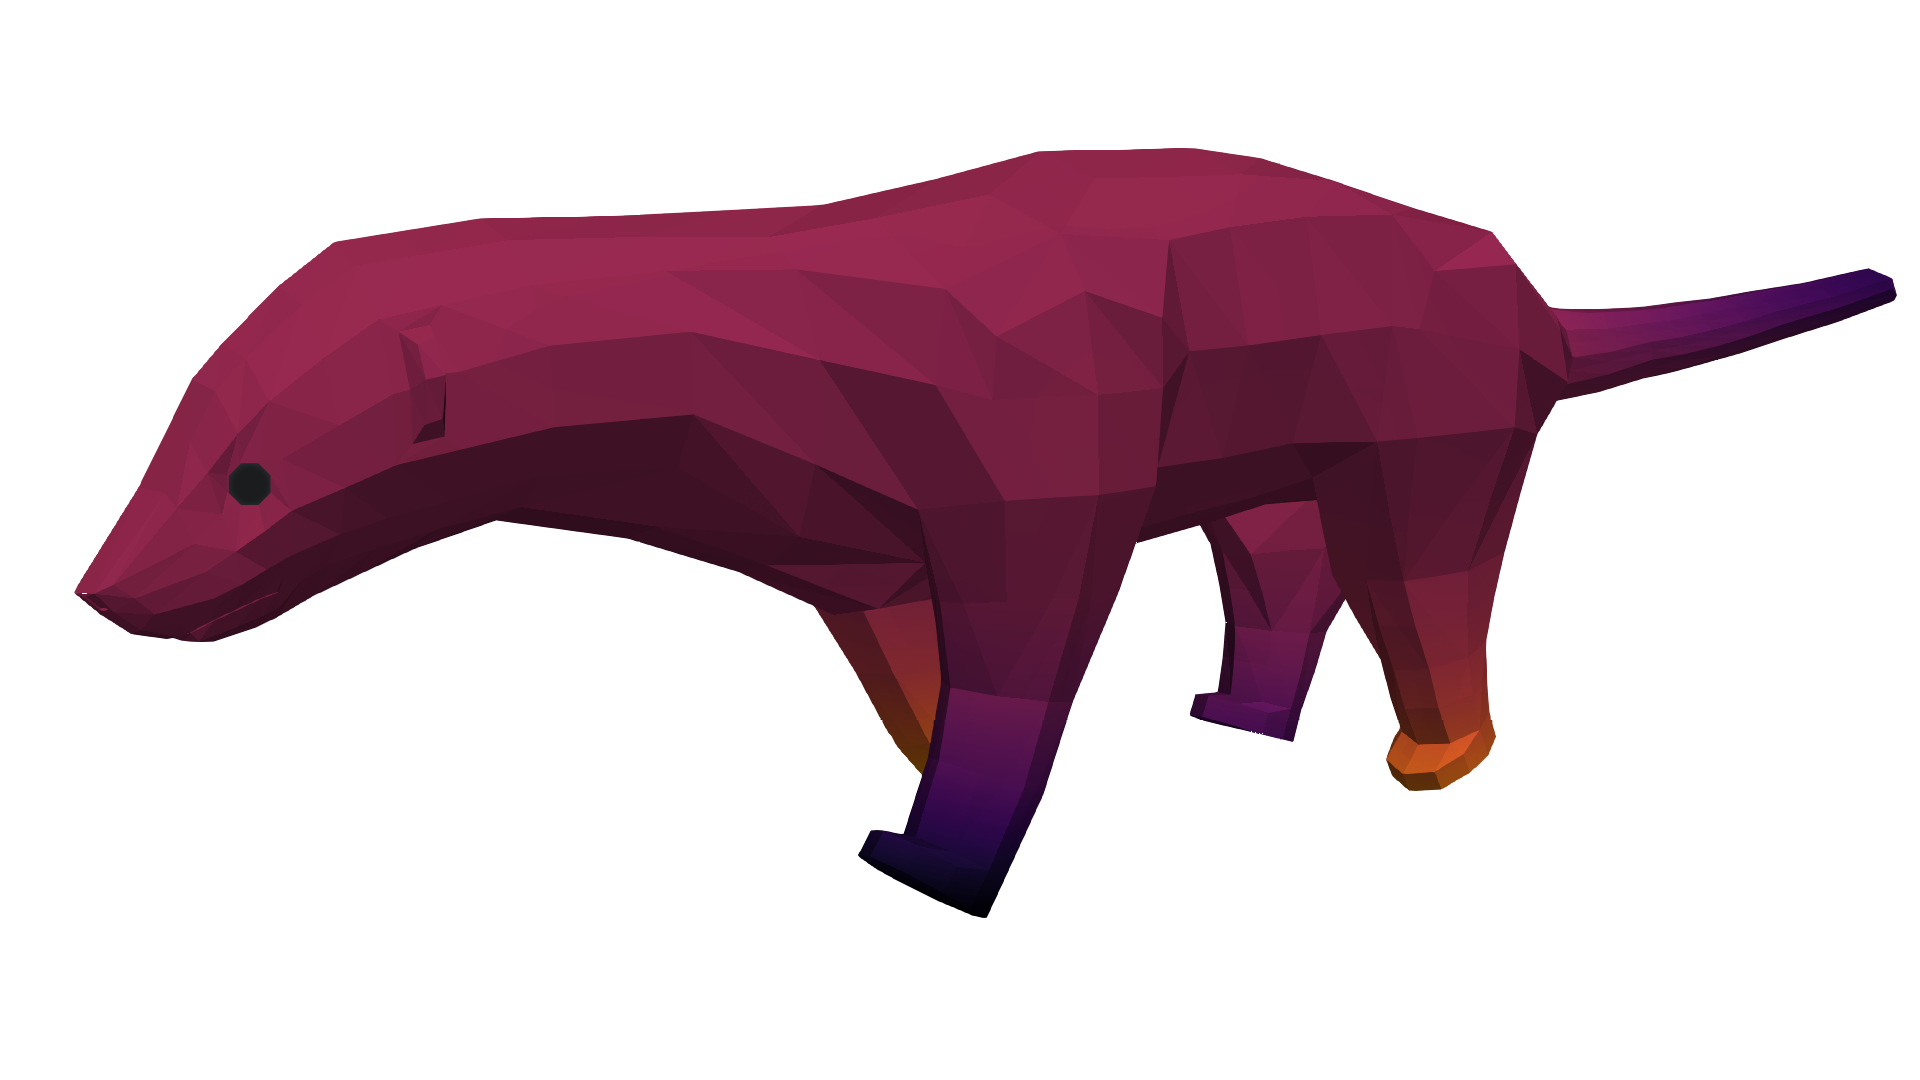
\includegraphics[height=2.75cm]{Ratellogo.png}
\end{center}

{\flushleft

Repository: https://gitlab.com/micromorph/ratel\\

~\\

Ratel Team: Zach R. Atkins, Jed Brown, Fabio Di Gioacchino,\\
\hspace{20mm} Leila Ghaffari, Zach Irwin, Rezgar Shakeri,\\
\hspace{20mm} Ren Stengel, Jeremy L Thompson\\

~\\

Grant: Predictive Science Academic Alliance Program (DE-NA0003962)\\

}

\begin{center}

\includegraphics[height=0.8cm]{psaap-center-logos}
\end{center}

\end{frame}

%-------------------------------------------------------------------------------

\end{document}

%-------------------------------------------------------------------------------
